\documentclass[a4paper]{article}

\usepackage[english]{babel}
\usepackage[utf8]{inputenc}
\usepackage{amsmath}
\usepackage{graphicx}
\usepackage[colorinlistoftodos]{todonotes}
\usepackage{titling}
\usepackage{listings}
\usepackage[T1]{fontenc}

\newcommand{\subtitle}[1]{%
  \posttitle{%
    \par\end{center}
    \begin{center}\large#1\end{center}
    \vskip0.5em}%
}
\lstset{%
  basicstyle=\scriptsize\sffamily,%
  commentstyle=\footnotesize\ttfamily,%
  frameround=trBL,
  frame=single,
  breaklines=true,
  showstringspaces=false,
  numbers=left,
  numberstyle=\tiny,
  numbersep=10pt,
  keywordstyle=\bf
}





%%%%%%%%%%%%%%%%%%%%%%%%%%%%%%%%%%%%%%%%%%%%%%%%%%%%
% Raport Headers:
%%%%%%%%%%%%%%%%%%%%%%%%%%%%%%%%%%%%%%%%%%%%%%%%%%%%





%%%%%%%%%%%%%%%%%%%%%%%%%%%%%%%%%%%%%%%%%%%%%%%%%%%%
% Rapport Headers:
%%%%%%%%%%%%%%%%%%%%%%%%%%%%%%%%%%%%%%%%%%%%%%%%%%%%
\title{Operating system. Synchronization Lab: Airport management}
\author{SID-LAKHDAR Riyane}
\date{20/11/2015}



\begin{document}
\maketitle

\begin{abstract}
	This document summarizes, refers and answers to the question of the fifth operating system laboratory: "Airport management".   All the required programs have been implemented and attached to this report.   All the implemented programs have been successfully compiled and tested (on the server "mandelbrot").   The compilation and running commands are given at the end of each section.   All the additional data structure that we implemented are in the file "sharedFile/shared.c/h".   This file is shared, during the compilation, with all the other repertories.
\end{abstract}


\section{One single runway, multiple planes}
In this question, there is a single runway.   This shared resource	 can only be accessed by a single thread at the time.\\
For this reason, we have chosen to synchronize our different threads thanks to a single lock mutex.  Our shared variable (runway) is implemented as a list where each thread appends its id.   This action is realized in a critical section.   The main thread launches all the threads and waits for all of them to finish them "landing".   This list has been implemented in the structure "runwayHistory".\\
Then the main thread checks this history list to print the id of the threads (plains) which have accessed (have landed) the resource.   It also checks whether the list has been corrupted (multiple simultaneous access to the shared resource).\\

The corresponding program has been implemented in the directory "question1".   It can be compiled using the command "make planeManager".   And it can be executed using the command "./planeManager <number of planes (non mandatory)>".

\section{Multiple runways, multiple planes}
Let's now consider the case where the shared variable may be accessed by at most N threads ($N \geq 1$) where N is the number of runways.   We have designed the access to this critical resource in a critical section based on a semaphore.   Thus, at each time, at most N thread can be simultaneously accessing the list of runways.\\

Among this N thread (in the critical section), we have also needed to synchronize an other critical resource which indicates which are the busy runways.  This resource can be accessed by a single thread at time.  Thus, it has been synchronized thanks to a single lock.  This critical section's nesting doesn't create deadlock because threads are not interdependent.   To make our synchronization test more representative, we have made each thread sleep (0.4 seconds).\\

The corresponding program has been implemented in the directory "question2".   It can be compiled using the command "make planeManager".   And it can be executed using the command "./planeManager <number of planes (non mandatory)> <number of runways (non mandatory)>".



\section{Multiple runways, multiple planes, FIFO access}
Once again, we are dealing with a critical section where N thread may be at the same time ($N \geq 1$).  Furthermore, this thread need to access the critical section in a "First in First out" order.   Thus, we have designed a waiting queue where each thread which wants to access write its id at the end of the queue.   The access to this shared queue is synchronized thanks to a mutex lock (at most one thread in this critical section).   The waiting thread are synchronized thanks to a condition variable.  Each time a thread gets out of the critical section, all the waiting thread are woke up through the condition variable.   The thread on the top of the queue (first arrived) is allowed to get into the critical section, while all the others sleep again.\\

The corresponding program has been implemented in the directory "question3".   It can be compiled using the command "make planeManager".   And it can be executed using the command "./planeManager <number of planes (non mandatory)> <number of runways (non mandatory)>".

\section{Multiple runways, multiple planes, priority between thread, FIFO access among a priority class}
For this question, the synchronizations needs are the same.   The only difference is that a new plane (thread) which asks for a runway (critical data) is not always appended at the end of the waiting queue.\\

The new waiting queue is built as shown in the figure Fig \ref{question4.png}.  A thread with a priority p is added after the last thread of priority p (if it exists) and before the first thread of priority p+1 (if it exists).\\

More formally, we have synchronized the access to waiting queue with a mutex lock (at most 1 thread in the critical section).  Once a thread has been appended in the waiting queue at the proper place, it starts waiting thanks to a condition variable.

\begin{figure}[ht!]
\center
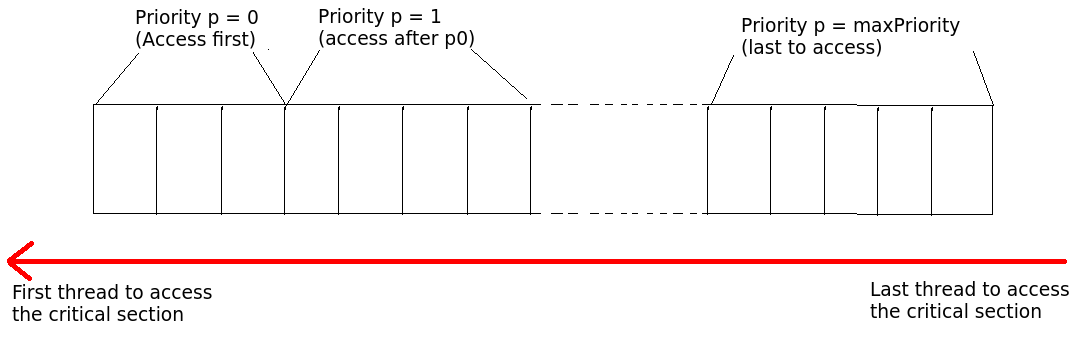
\includegraphics[width=0.8\linewidth]{question4.png}
\caption{Priority waiting queue with sort among priority classes.}
\label{question4.png}
\end{figure}



\end{document}


